\documentclass[12pt,a4paper]{article}

\usepackage[utf8]{inputenc}
\usepackage[T1]{fontenc}
\usepackage[francais]{babel}
\usepackage{setspace}
\usepackage{graphicx}

\title{Diagramme d'architecture}

\author{Hereiti \bsc{Hatitio} - Anta \bsc{Mbaye} - Maxime \bsc{Vincent} - Jean-Baptiste \bsc{Rey}}

\begin{document}
\maketitle

\newpage
\vspace*{-1in}
\vspace*{-\the\hoffset}
\thispagestyle{empty}
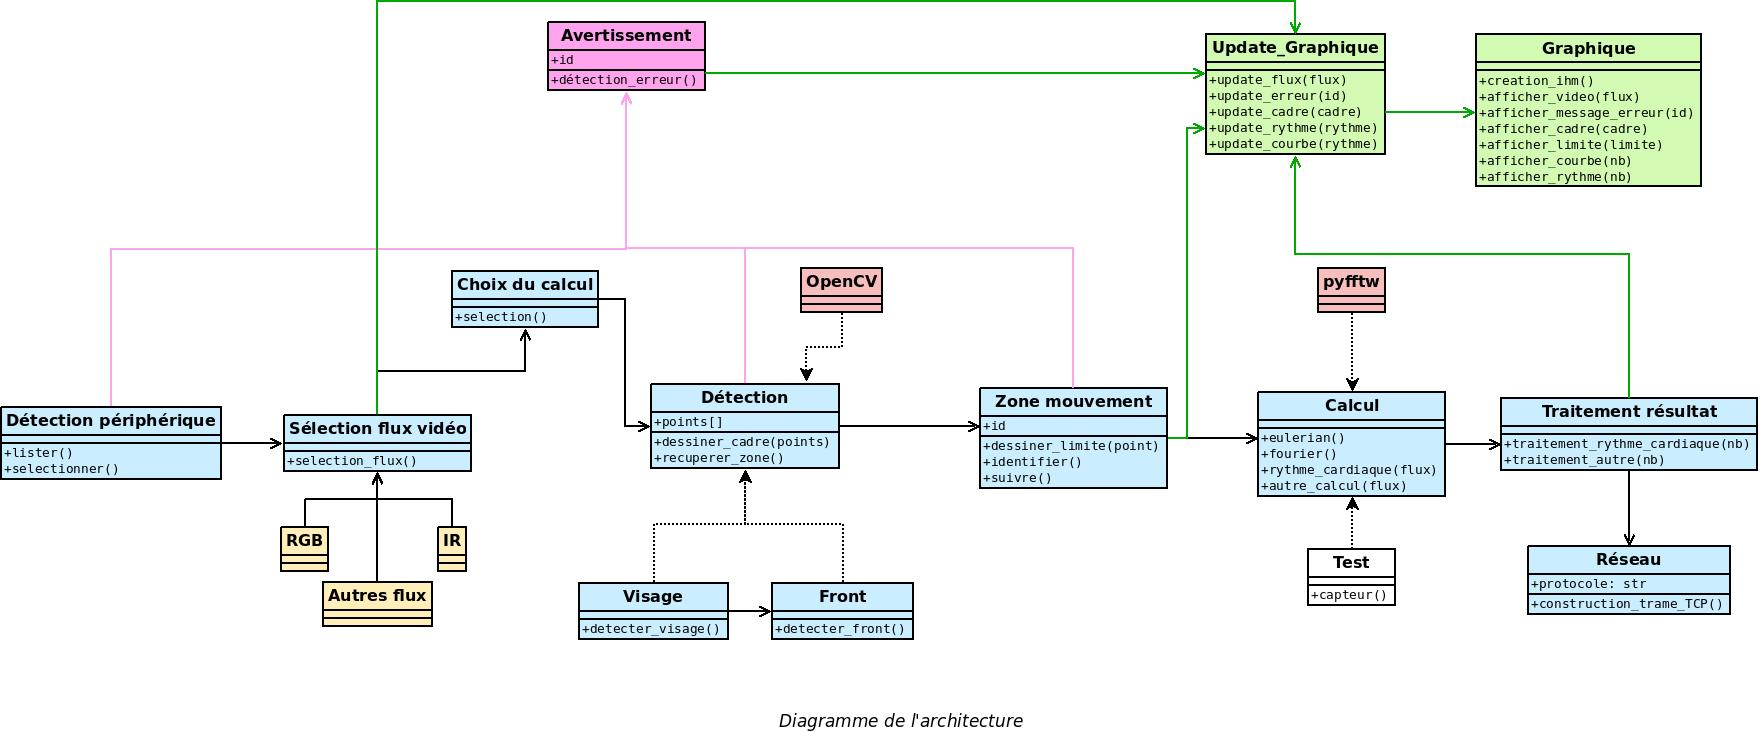
\includegraphics[scale=0.4,angle=90]{archi2.jpeg}
\begin{center}

\end{center}

\includegraphics[scale=0.5]{bleu.png} : Modules implémentant besoins fonctionnels\newline
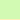
\includegraphics[scale=0.5]{vert.png} : Module d'affichage graphique\newline

\includegraphics[scale=0.5]{orange.png} : Flux vidéo\newline

\includegraphics[scale=0.5]{rouge.png} : Framework\newline

\includegraphics[scale=0.5]{rose.png} :  Module de traitement des erreurs

\subsection*{Détection périphériques}

Dans ce module, on liste les différents périphériques utilisables. Et on permet d'en sélectionner un.

\subsection*{Récupérer flux vidéo}

Dans ce module on sélectionne le flux (RGB, IR ou autres) pour appliquer le tracking. Il sera ensuite affiché dans l'IHM.


\subsection*{Choix du calcul}



\subsection*{Détection}
A l'aide d'OpenCV, ce module permet de détecter la zone de traitement suivant un choix de l'utilisateur, puis de dessiner le cadre de cette zone.

\subsection*{Zone mouvement}

Ce module délimite la zone de mouvent possible sans perte de tracking. Il identifie également les utilisateurs par un ID numérique. Si un utilisateur sort de son cadre, le tracking est perdu, il est repris que lorsqu'une nouvelle zone de traitement est détecté.

\subsection*{Avertissements}
En cas d'erreurs produit par les différents modules précédents, un message s'affiche sur l'IHM spécifiant l'erreur.

\subsection*{Autre traitement}

Ce module est imaginé en cas de nouveau traitement à appliqué sur la zone de traitement. Par exemple, la mesure du rythme respiratoire peut être imbriqué à cette endroit dans notre programme.

\subsection*{Calcul rythme cardiaque}

Ce module permet le calcule en boucle du rythme cardiaque tant qu'une zone de traitement est valide. 
En cas de plusieurs utilisateurs, le même algorithme est utilisé plusieurs fois.



\subsection*{Afficher résultat}

Le résultat du traitement précédent est envoyé à l'IHM, qui l'affiche sous forme de train binaire ou de courbe suivant le choix de l'utilisateur.

\subsection*{Réseau}

De même que précédemment, le résultat du traitement peut être envoyé sur le réseau dans une trame TCP. Le choix du protocole(OSC ou LSL) sera déterminé par l'utilisateur.




\end{document}